\documentclass[a4paper]{article}

\usepackage{a4wide}
\usepackage[utf8]{inputenc}
\usepackage[T1]{fontenc}
\usepackage{graphicx}
\usepackage{float}

\bibliographystyle{alpha}

\begin{document}

\title{Explanation Architecture for Companion Systems}
\author{Tamino Hartmann}
\date{\today}

\maketitle
\newpage

\tableofcontents

\newpage

\section{Introduction}

When users buy a new electronic device such as a smartphone, they often look at the advertised features listed on the box. Most pick out the few features that are important to themselves while others simply compare the length of the list. However even if a user buys a new smartphone for a new feature, the purchase does not come with an instant understanding of the feature. Once unpacked at home, the user is then faced with finding the feature and learning to use it – a task that is often not without its problems. If the hurdle is deemed too large, the new gadget is perceived to be a disappointment. Said frankly, you could say that the user is unwilling to cooperate with the device.

Changing this is the main purpose of the paper "Explanation Architecture for Companion Systems"\cite{origin}. It expands on the idea of providing an explanation architecture, primarily for systems that offer a user dialogue. The aim of providing explanations is to strengthen a user's willingness to work with the system to solve problems or complete tasks. Apart from simply explaining new things to a user, such a system can also be used to cooperate with a user on tasks such as creating the user's calendar with given constraints such as time restrictions and travel times.

The original paper concentrates on so-called companion systems. Companion systems are systems that assist a user in a multitude of day-to-day tasks, such as the aforementioned scheduling of appointments. However, the capabilities of a companion system do not stop there. Using a vast array of knowledge, these systems can also help a user with a new and unknown task, tasks that are out of a user's comfort zone. To make the most of such a system, this architecture is deployed using a range of modules, so as to make it easy to include any available device to help the user. However, the core system should be based upon a device that the user keeps with her the entire day. This could, for example, be a smartphone\footnote{TODO: Add an example? (attach beamer to smartphone for showing map or something like it?)}. It is important to point out that companion systems here are not understood to be static programs; instead, they attempt to adapt to a user's preferences, behavior, knowledge, and emotional state. Apart from that they can also adapt to external influences such as time of day, situation, and any other information at disposal to the system.

However, it must be asked whether such a system is even feasible at the current level of technology. The system developed in the original paper is a proof of concept to this. Every year new advances allow companion systems to evolve from simple programs presenting plain static information to a system capable of holding a dialogue with a user while reacting to any input it can get its hands on. To make such a dialogue more and more realistic it becomes progressively more important to include a way for the system to explain things to a user, be that to present a reason for a decision or to further the knowledge of a user. In the future such companion systems might well make decisions for a user completely autonomously, based only on gathered working knowledge of the user.

The first issue that influences a cooperation between a user and the system is a user's knowledge of system features and capabilities. This can be done for example by adapting the user interface based upon whether the user is a novice or an expert, beyond simply providing helpful functions and tutorials.

Another issue is when the system does something that the user can not comprehend because she lacks information or knowledge. This can be dangerous to the trust the user extends towards the system, as a decrease of transparency can have ill effects, such as a decrease of using the system down to not using the system at all. The reason for this is that humans tend to only accept someone's decisions only when the reasons behind them are clear to them. This is a byproduct of a human's natural autonomy. This leads the original paper to come to the conclusion that especially in companion systems, the issues surrounding trust between a user and the system are increasingly important to uphold a user's willingness to interact with the system, which might even prevent the companion system from being used at all.

\section{Trust}

In the introduction, we reflected upon the effect of trust between a user and a companion system. To understand the problem and the solution, it is important to understand what "trust" is in this context. Several definitions exist, with the following one being the one used most frequently: trust is when one party (referenced as the trustor) is thought to be in a vulnerable situation by relying completely upon the actions of a second party (referenced as the trustee). Trust is not only an aspect to consider when looking at human interactions; trust is also relevant for the interaction between a user and a system\footnote{TODO: Source?}. A definition of trust adapted to usage between a user and the system is: the extent to which a user is confident in, and willing to act on the basis of, the recommendations, actions, and decision of an artificially intelligent decision aid\cite{htc}. This definition is used because it includes but distinguishes between both the user's confidence in a system and the user's willingness to use the system to solve a problem.

Companion systems of course contain decision aid systems, but they can do even more. Simply showing information as happens with a help function does not necessarily solve the problem of an uncooperative user. This is because to understand a decision or an action the system has taken, the user does not need an understanding of the concepts involved, instead she requires an understanding of the process that lead to the decision or action. That is a fine but important distinction; not the knowledge behind the decision, but the reasons for the decision are important. This shows that not the unknown quality of a companion systems knowledge is important for trusting, but the reasoning based on the knowledge.

It becomes clear that one of the most elementary things a companion system can do to strengthen the trust between itself and a user is providing adaptive explanations. Perceived trust is not easy to describe as a concept; it consists of several influential parts based on intentions, motives, and actions of the two parties. To counter trust issues, it is necessary to know what parts of the concept have to be addressed. For that to happen, the base concepts must be explored.

For human trust relationships, the original paper references \cite{htc}. In it, trust is defined in three levels: ability, integrity, and benevolence. Ability describes the capacity to do something based on competencies, skills, and the characteristics of the trustee. Integrity describes perceived moral uprightness of the trustee by the trustor. Benevolence describes the disposition to do good for the trustor.

\begin{figure}[H]
	\centering
	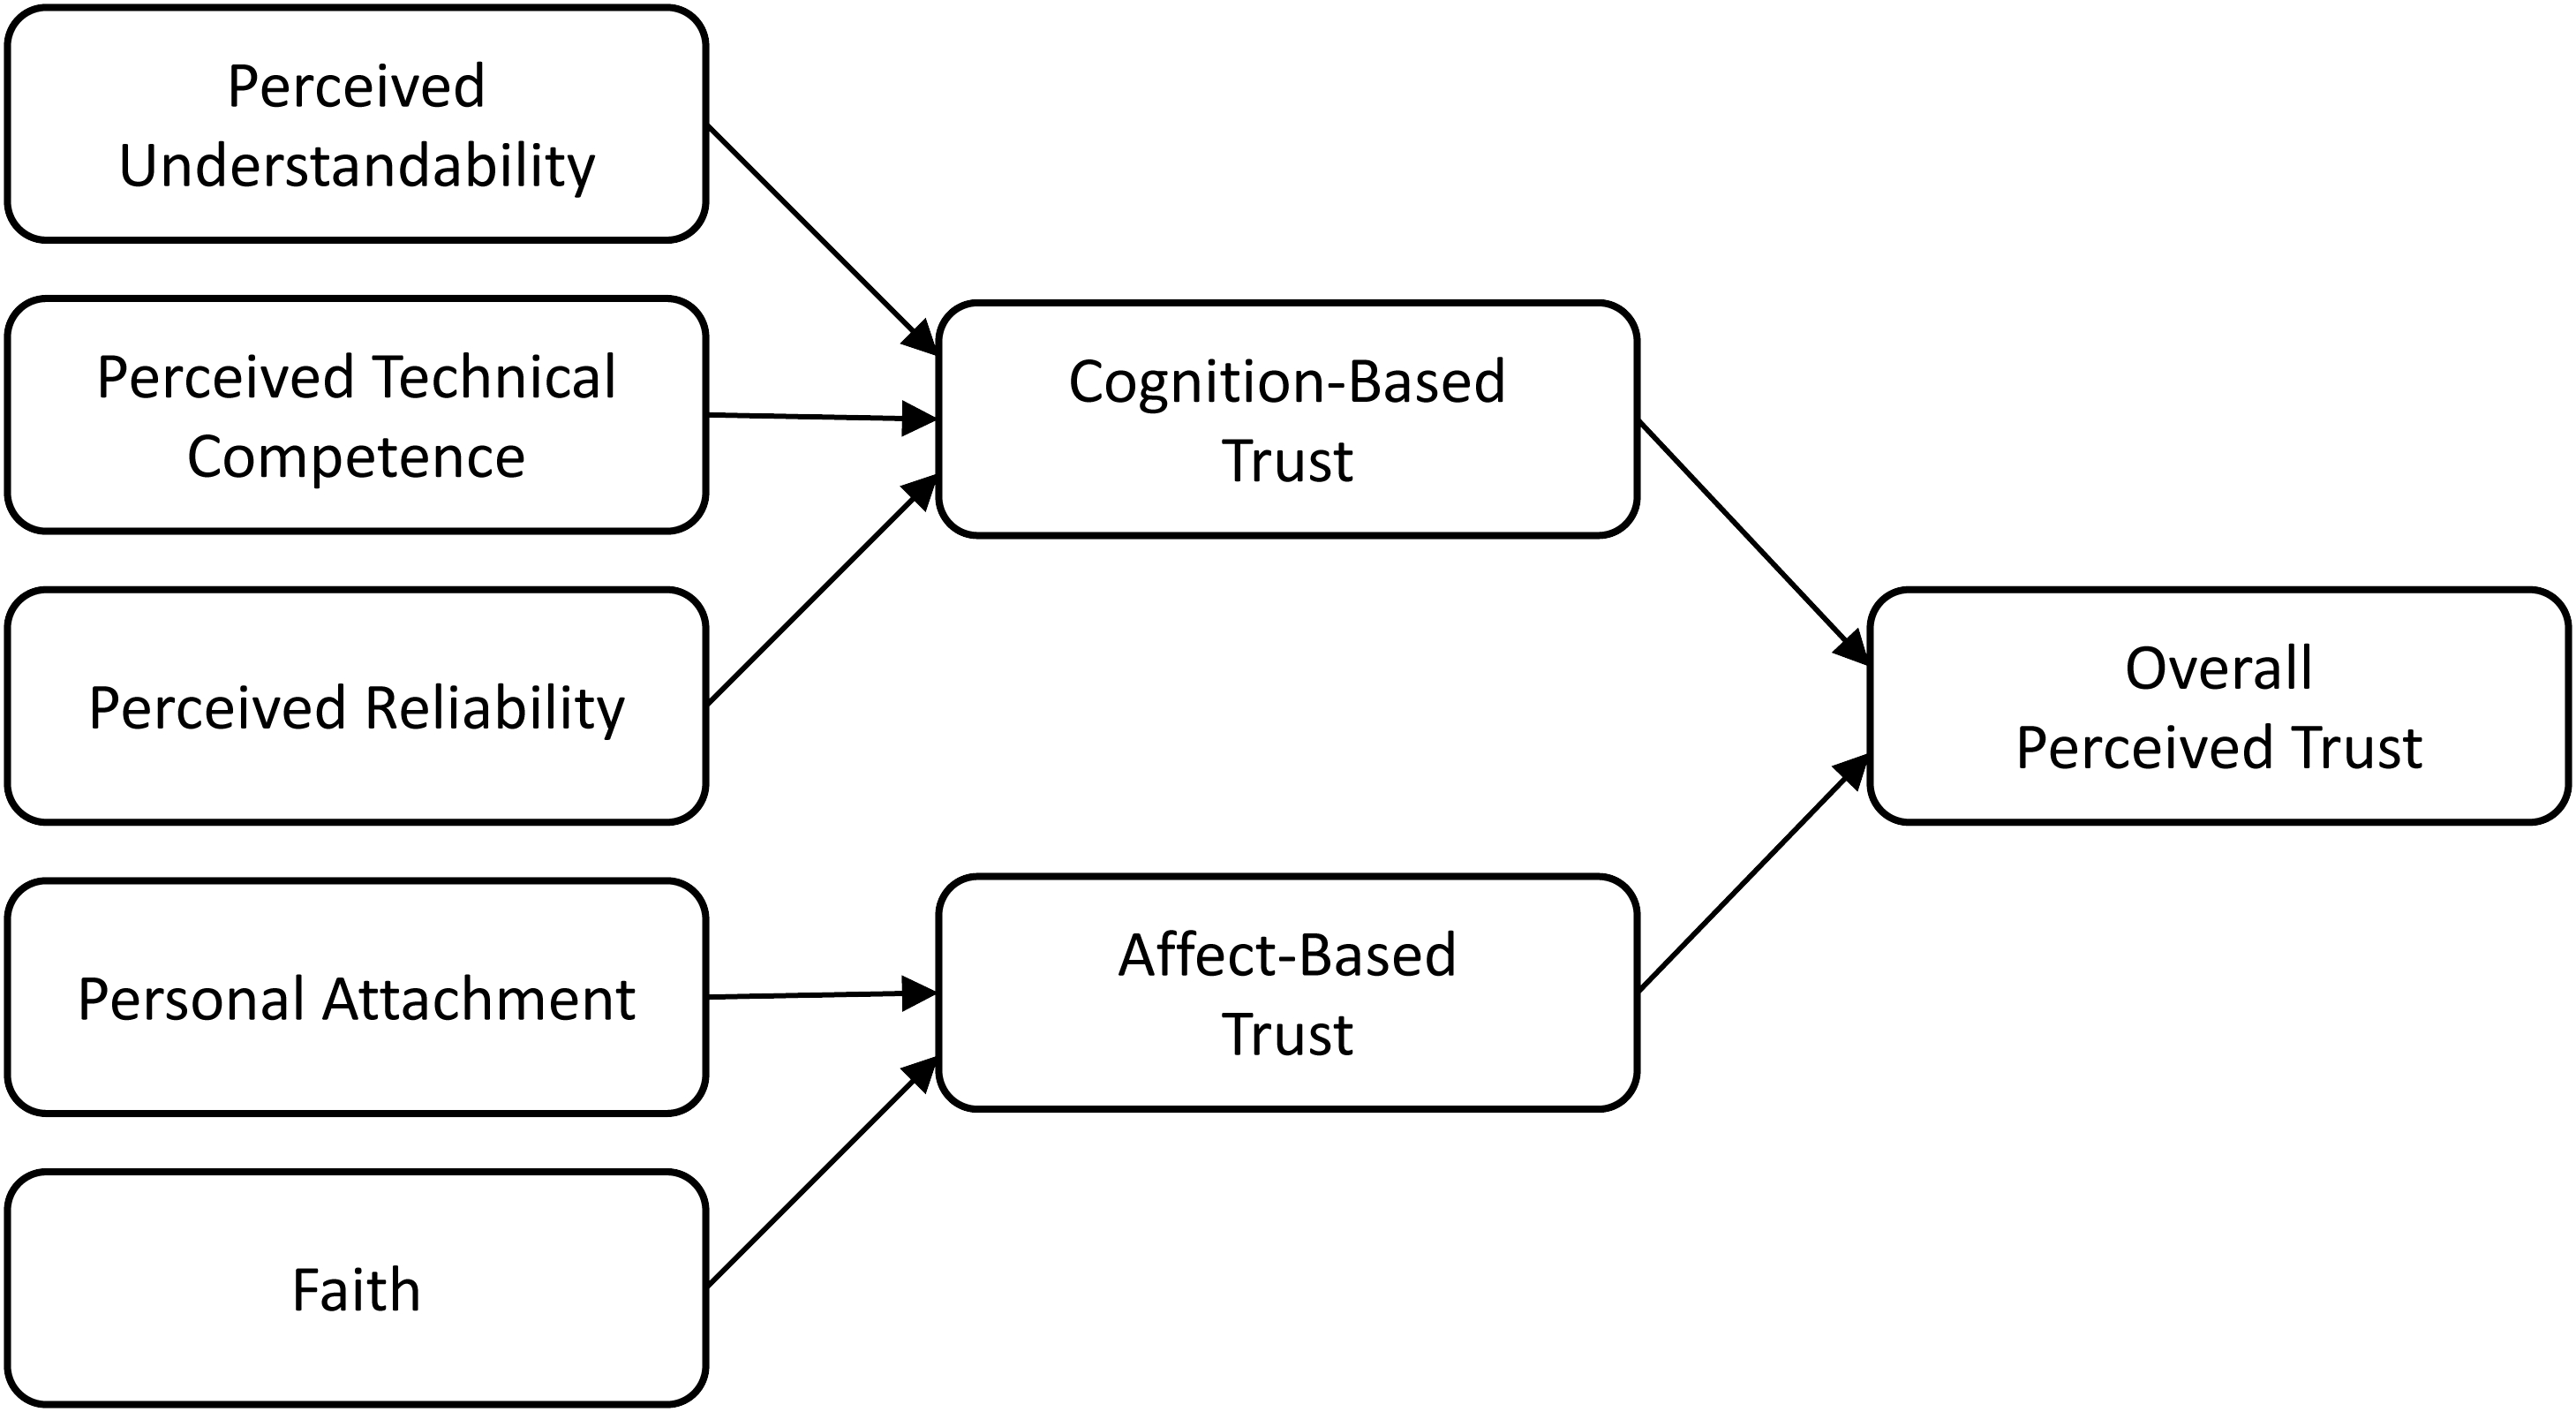
\includegraphics[width=10cm]{trust.png}
	\caption{This is the human-system trust model upon which the original paper founds its explanations.}
	\label{fig:hs_trust}
\end{figure}

For a human-system trust relationship, trust can be separated into nine basic constructs as seen in Figure \ref{fig:hs_trust}. Note that four constructs are left out due to representative and discriminative issues. This gives us five basic constructs of trust with which to work. Concerning the overall perceived level of trust, all five constructs must be perceived to be high. If just a single one is low, the overall trustworthiness suffers. Given that we require working knowledge of the level of trust, we need to know the levels of trust that the trustor is perceiving. This proves to be difficult though because they can only be measured with a questionnaire, which is not something a companion system can do whenever trust must be measured.

To enable a companion system to at least have a broad grasp of the measure of trust, the original paper employs reinforcement learning. With it, the system tries to find a solid trade-off between the exploitation of knowledge and the exploration of new aspects. Reinforcement learning is an area of machine learning that tries to teach a system to take actions based on the goal of a perceived reward. Here, the goal likely is a higher level of trust as recognized by the companion system.

In the original paper, these decisions are made based on handcrafted policies, as a statistical approach is not viable due to a lack of data. In the future, these handcrafted policies can probably be replaced by data collected from a multitude of users, possibly in a non-static way so that the data is always expanding.

\section{Countering Trust Issues}

Given that we now have a measure of trust, the next step in solving a trust issue is how to counter it. In the original paper, this is done solely by applying explanations to a situation. Simply explaining everything is not the way to do that, however – too much explanations make the usage of a companion system more a hurdle than a plus, as they could lengthen the solving of a problem with unneeded dialogue. This means that we need to know two things: what problems a user will normally face while using a companion system and which events should trigger an explanation.



\section{Explanations}

explain explanation (transfer of understanding in a dialogue system in which a questioner and a respondent take part)

\subsection{Selecting Explanations}

problem of selecting appropriate type of explanation

types of explanation can follow several or only one goal of explanation

strategies for selecting appropriate explanation

???

\subsection{Where to Use Explanations}

events that start the process of providing explanations

done with knowledge base

comparison of user knowledge base with conceptual knowledge required

various aspects of knowledge graphs used

decay over time, etc...

\section{Architecture}

modular

show / explain graph

using inter-system api modules can interact with each other

each module works completely autark from others, only respond to events (like “need explanation”)

[show path of explanation through system as summary?]

\section{Conclusion}

affirm decision of why explanations are required and useful

handling of trust issues needs to be refined

important(?): explanations can be adapted by any module in the system to fit the need

\newpage

\bibliography{doc}

\end{document}